\chapter{Homotopies}\label{chp:4_1}

Recall that a path is a continuous function $a : [0, 1] \rightarrow X$. 
The idea here is that we have two paths $a_0$ and $a_1$ in $R^2$ 
with $a_0(0) = a_1(0)$ and $a_0(1) = a_1(1)$;
i.e. the paths have the same endpoints.

\begin{figure}[H]
    \centering
    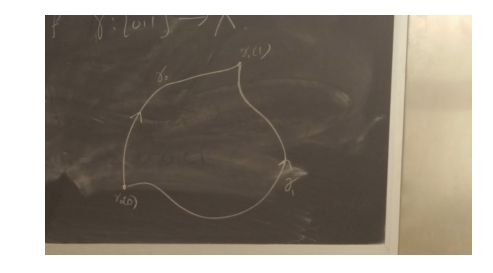
\includegraphics[width=0.6\textwidth]{figure/homotopy1.png}
    \caption{}
\end{figure}

Our paths are different and may even have different images, but we want to say that one
can be continuously deformed into the other.

\begin{figure}[H]
    \centering
    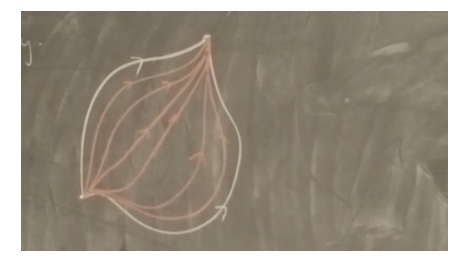
\includegraphics[width=0.6\textwidth]{figure/homotopy2.png}
    \caption{}
\end{figure}

Intuitively, we want to create a family of paths $\{a_t\}_{t\in[0,1]}$ “from $a_0$ to $a_1$.” 
You can also say we want to interpolate continuously between $a_0$ and $a_1$. 
Think of $\{a_t: t \in [0, 1]\}$
as one function $a : [0, 1] \times [0, 1] \rightarrow X$, 
where $a(x, t) := a_t(x)$.


The notion $C(X,Y)$ is the set of all the continuous maps from $X$ to $Y$.

Two continuous functions from one topological space to another are called homotopic if one can be “continuously deformed” into the other, such a deformation being
called a homotopy between the two functions. More precisely, we have the following
definition.

\begin{definition}{}{}
    Let $X, Y$ be topological spaces, and $f, g : X \rightarrow Y$ continuous maps.
A homotopy from $f$ to $g$ (denoted by $H: f\simeq g$) is a continuous function $H : X \times [0, 1] \rightarrow Y$ satisfying
$H(x, 0) = f(x)$ and $H(x, 1) = g(x)$, for all $x \in X$.
If such a homotopy exists, we say that $f$ is homotopic to $g$, 
and denote this by $f\simeq g:X\rightarrow Y$ or $f\simeq g$. 
\end{definition}

\begin{definition}{}{}
    If $f$ is homotopic to a constant map, i.e., if $f \simeq \text{const}_y$, 
for some $y \in Y$ , then we say that $f$ is nullhomotopic.
\end{definition}

\begin{proposition}{}{}
    Let $f, g : E^n \rightarrow E^n$ any two continuous, real functions. 
    Then $f \simeq g$. 
\end{proposition}
To see why this is the case, 
define a function $F : E^n \times [0, 1] \rightarrow E^n$ by
$H(x,t)=(1-t)\cdot f(x)+t\cdot g(x)$.
$H$ is continuous and $H(x,0)=f(x),H(x,1)=g(x)$. 
Thus, $H$ is a homotopy between $f$ and $g$.

\begin{proposition}{}{}
    Let $A$ be a convex subset of $E^n$, endowed with the subspace topology,
and let $X$ be any topological space. Then any two continuous maps $f, g : X \rightarrow A$ are
homotopic. The homotopy from $f$ to $g$ called the straight line homotopy.
\end{proposition}

\begin{proposition}{}{}
    If $Y$ is convex, $p \in Y$ , $f : X \rightarrow Y$ 
    is continuous, and $g : X \rightarrow Y$ is $g(x) = p$
    for all $x \in X$, then $f \simeq g$ via the straight line homotopy.
\end{proposition}



\begin{proposition}{}{}
    Homotopy is an equivalence relation on $C(X, Y)$.
\end{proposition}

\begin{proposition}{}{}
    If $f_0\simeq f_1: X\rightarrow Y$,
    $g_0\simeq g_1:Y\rightarrow Z$, then
    $g_0\circ f_0\simeq g_1\circ f_1:X\rightarrow Z$.
\end{proposition}

\begin{proposition}{}{}
    Let $y_1,y_2\in Y$ and $f_{y_i}:X\rightarrow Y$ given by $f(X)=y_i$.
    Then $f_{y_1}\simeq f_{y_2}\Leftrightarrow$ $y_1$ and $y_2$ is in the same path component.
\end{proposition}


\begin{proposition}{}{}
    If $Y$ is path-connected, then the set $[I,Y]$ 
    (the homotopy classes of maps from $I$ to $Y$) 
    has a single element.
\end{proposition}


For our paths, we want to fix the start and end, so $a_t(0) = a_t(1) = a_0(1)$ for all $t \in [0, 1]$.

\begin{definition}{}{}
    Let $A\subseteq X$ and $f,g\in C(X,Y)$.
    We say $f$ and $g$ are homotopic relative to $A$ iff there exists a homotopy $H$ between $f$ and $g$, and:\\
    (1) $\forall a\in A$: $f(a)=g(a)$\\
    (2) $\forall a\in A, t\in [0,1]$: $H(a,t)=f(a)$\\
    and denote this by $f\simeq g \text{ rel}A$ and $H:f\simeq g\text{ rel}A$.
\end{definition}

\begin{proposition}{}{}
    If $A\subseteq X$, homotopy relative to $A$ is an equivalence relation on $C(X, Y)$.
\end{proposition}

\begin{proposition}{}{}
    If $f_0\simeq f_1: X\rightarrow Y \text{ rel}A$,
    $g_0\simeq g_1:Y\rightarrow Z\text{ rel}B$ and $f_0(A)\subset B$, then
    $g_0\circ f_0\simeq g_1\circ f_1 \text{ rel}A$.
\end{proposition}

\begin{definition}{}{}
    Let $a$ and $b$ be paths in $X$. $a$ is path-homotopic to $b$ if $a\simeq b \text{ rel}\{0,1\}$
    and denoted by $a \underset{\cdot}{\simeq} b$. i.e.
    there exists a homotopy $H$ between $a$ and $b$ such that:\\
    (1) $a(0)=b(0),a(1)=b(1)$\\
    (2) $\forall t\in [0,1]$: $H(0,t)=a(0), H(1,t)=a(1)$.
\end{definition}

\begin{figure}[H]
    \centering
    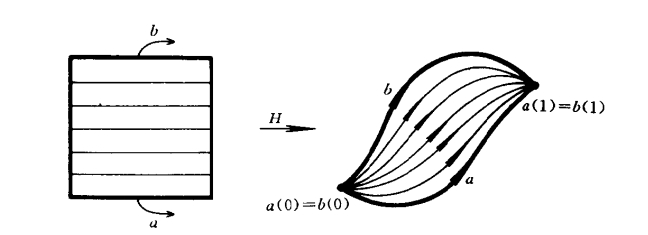
\includegraphics[width=0.6\textwidth]{figure/path-homotopic.png}
    \caption{}
\end{figure}

Since homotopy relative to a subset is an equivalence relation, 
it follows that path-homotopy is a equivalence relation on the set $P(X)$ of all paths in $X$.
Then path-homotopy be a partition of $P(X)$ into
disjoint subsets whose union is $P(X)$. These disjoint subsets are called path classes in $X$.
The collection of all path classes is denoted by $[X]$.
Given path $a$, the path classes $a$ belongs to denoted by $<a>$.
The startpoint and endpoint of $a$ are the startpoint and endpoint of $<a>$.
The path class is call closed path class if its startpoint and endpoint coincide, 
then its startpoint(endpoint) is called base point.


\section{Reference}
\begin{itemize}
    \item \href{https://www.math.toronto.edu/~herzig/MAT327-lecturenotes21b.pdf}{Path Homotopy}
    \item \href{https://www.ms.uky.edu/~guillou/F17/551Notes-Week15.pdf}{Path-homotopy}
    \item \href{http://staff.ustc.edu.cn/~wangzuoq/Courses/21S-Topology/Notes/Lec18.pdf}{HOMOTOPY AND PATH HOMOTOPY}
    \item \href{https://pillowmath.github.io/Math%20142/Lec9.pdf}{Homotopy}
\end{itemize}